\section{Języki pełnościeżkowe}% (fold)
\label{sec:jezyki_pelnosciezkowe}
\newcommand{\Elisc}{\ensuremath{\mathrm{E}^{\textrm{liść}}}}


\begin{definicja}
	Język pełnościeżkowy to booleowska kombinacja języków postaci
	$$\Elisc L.$$
\end{definicja}

Sformułujemy teraz twierdzenie analogiczne do \ref{tw:sciezkowe}, charakteryzujące języki pełnościeżkowe poprzez ich algebrę syntaktyczną. Zauważmy najpierw, że twierdzenie w wersji dla języków ścieżkowych to rzeczywiście zbyt mało --- problematyczna jest tu równość $(ii)$: gdy za $g$ podstawimy pusty las otrzymamy:

$$v(0+h) = v0 + vh,$$

czyli

$$vh = v0 + vh.$$

Od razu widać, że ta równość niekoniecznie musi być spełniona, gdyż zbiór \textit{ścieżek liściowych} (pełnych ścieżek korzeń -- liść) prawej strony równości może być istotnie większy od zbioru pełnych ścieżek lewej strony.

Musimy więc nieco wzbogacić to twierdzenie, co uczynimy poniżej.

\begin{twierdzenie}
	Niech $L \subseteq H_A$ będzie regularnym językiem lasów. Niech $(H_L, V_L)$ będzie jego algebrą syntaktyczną. Następujące warunki są równoważne:
	
	\begin{enumerate}[(a)]
		\item $L$ jest językiem pełnościeżkowym
		\item $(H_L, V_L)$ spełnia:
		\begin{enumerate}[(i)]
			\item $h + g = g + h$ dla $h,g \in H_L$\label{(i)}
			\item $v(g+h) = vg + vh$ dla $v \in V_L$, $g,h \in H_L$, o ile $g,h$ są obrazami niepustych lasów\label{(ii)}
			\item $h + h = h$, dla $h \in H_L$.\label{(iii)}
		\end{enumerate}
	\end{enumerate}
\end{twierdzenie}

Poczyńmy kilka obserwacji:

\begin{fakt}
	Tak jak w przypadku języków ścieżkowych, równanie (\ref{(iii)}) jest konsekwencją równań (\ref{(i)}) oraz (\ref{(ii)}).
\end{fakt}

\begin{fakt}\label{fakt:homomorfizm}
	W odróżnieniu od języków ścieżkowych, rozstrzygnięcie czy dany język jest językiem pełnościeżkowym wymaga badania nie tylko algebry syntaktycznej, ale też homomorfizmu syntaktycznego.
\end{fakt}

Zatrzymajmy się na chwilę nad faktem \ref{fakt:homomorfizm}. Zauważmy, że modyfikacja twierdzenia \ref{tw:sciezkowe} polegała na dodaniu do równości (\ref{(ii)}) założenia ,,o ile $g,h$ są obrazami niepustych lasów''. Rzeczywiście opisuje to homomorfizm, a nie algebrę. Aby zilustrować ten fakt, przyjrzyjmy się następującemu przykładowi.

\begin{przyklad}
	Przedstawimy dwa języki spośród których tylko jeden jest językiem pełnościeżkowym. Oba za to mają taką samą algebrę syntaktyczną.
	
	\begin{itemize}
		\item $L = \textrm{,,istnieje liść $a$''}$, $A = \{a,b\}$,
		\item $L' = \textrm{,,po usunięciu $c$ istnieje liść $a$''}$, $A = \{a,b,c\}$.
	\end{itemize}
	
	Przez ,,usunięcie $c$'' rozumiemy następującą operację:
	
	\begin{center}
		\begin{minipage}[t]{.25\linewidth}
			\vspace{0pt}
			\centering
			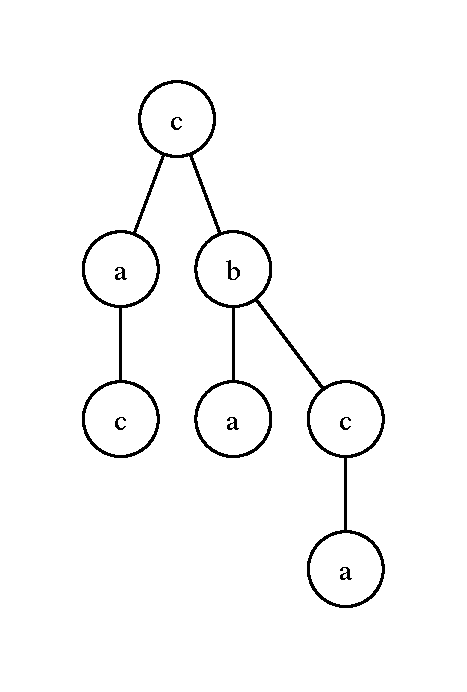
\includegraphics[scale=0.6]{rysunki/w12-usuniecie_c_1.pdf}
		\end{minipage}
		\begin{minipage}[t]{.25\linewidth}
			\centering 
			\vspace{40pt}
			\begin{displaymath}
				\xymatrix{ 
					\ar@{~>}[rr]^{\textrm{usunięcie $c$}} &&
				}
			\end{displaymath}
		\end{minipage}
		\begin{minipage}[t]{.25\linewidth}
			\vspace{0pt}
			\centering
			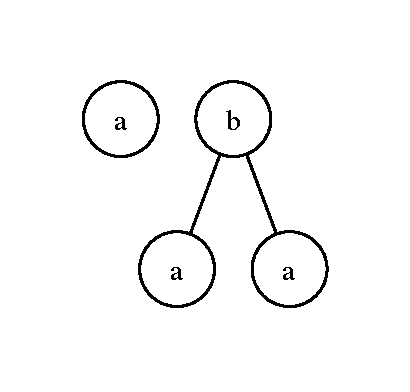
\includegraphics[scale=0.6]{rysunki/w12-usuniecie_c_2.pdf}
		\end{minipage}
	\end{center}

	Oczywiście $L$ jest językiem pełnościeżkowym. Oba te języki mają taką samą algebrę syntaktyczną --- danemu $t' \in L'$ przypisany jest ten sam element algebry co odpowiadającemu mu $t \in L$ (tzn. osiągniętemu przez usunięcie $c$).

	$L'$ nie jest za to językiem pełnościeżkowym. Rozpatrzmy przedstawione poniżej lasy $t_1$ (po lewej) oraz $t_2$. Odpowiadający im zbiór ścieżek liściowych jest taki sam, ale $t_1 \in L'$, a $t_2 \notin L'$.

	\begin{center}
		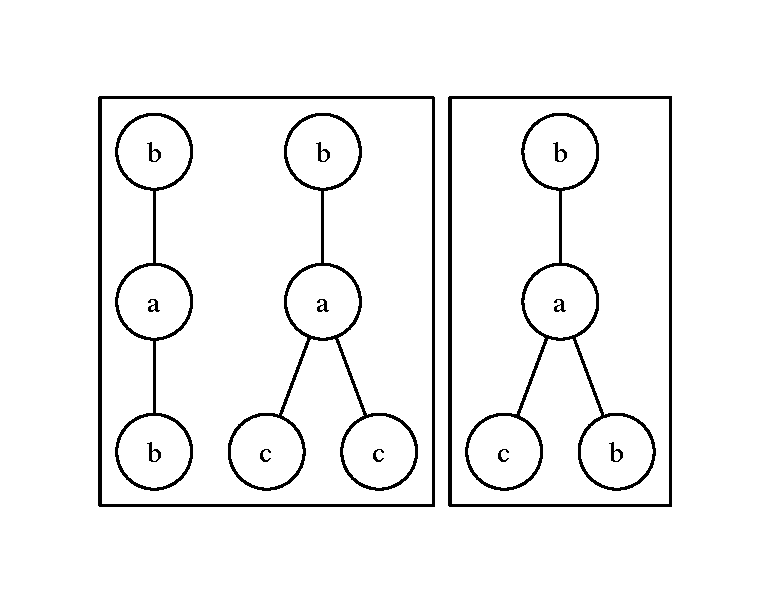
\includegraphics[scale=0.6]{rysunki/w12-l_prim.pdf}
	\end{center}

\end{przyklad}
% section języki_pełnościeżkowe (end)

\section{Logika temporalna} % (fold)
\label{sec:logika_temporalna}

\newcommand{\LTL}{\ensuremath{\mathtt{LTL}}}
\newcommand{\CTL}{\ensuremath{\mathtt{CTL}}}
\newcommand{\CTLS}{\ensuremath{\mathtt{CTL*}}}
\newcommand{\opA}{\ensuremath{\mathrm{A}}}
\newcommand{\opE}{\ensuremath{\mathrm{E}}}

\textit{Logika temporalna} to logika na drzewach (nieurangowanych) podobna do $\LTL$. Będziemy rozpatrywać dwa typy tej logiki: $\CTL$ oraz $\CTLS$. Ta ostatnia ,,mniej więcej'' odpowiada $FO$ (co oznacza ,,mniej więcej'' zostanie wyjaśnione na kolejnych wykładach). Ponadto zachodzi

$$\CTL \subsetneq \CTLS.$$

\subsection{Przykłady} % (fold)
\label{sub:przyklady}

Zanim przystąpimy do definicji, przeanalizujmy kilka przykładów.

\begin{przyklad}
	$L = \textrm{,,istnieje ścieżka na której występuje $a$''}$ można opisać jako

	$$\opE F^*a.$$
\end{przyklad}

\begin{przyklad}
	$L = \textrm{,,istnieje wierzchołek $b$ który ma samych przodków $a$''}$ można opisać jako

	$$\opE b U a.$$
\end{przyklad}

\begin{przyklad}
	$L = \textrm{,,po usunięciu $c$ istnieje liść $a$''}$ (język $L'$ z poprzedniego rozdziału) można opisać jako

	$$\opE F^*(a \land \opA XGc).$$
\end{przyklad}

\begin{przyklad}
	$L = \textrm{,,istnieje ścieżka liściowa $(ab)^{+}c$''}$ można opisać jako

	$$\opE a \land G(a \Rightarrow Xb) \land G(b \Rightarrow X(a \lor c)) \land G(c \Rightarrow \neg X T).$$
\end{przyklad}

% subsection przykłady (end)

\subsection{Składnia} % (fold)
\label{sub:skladnia}

W tym paragrafie sformułujemy formalnie składnię logiki temporalnej.

Zauważmy, że konstruując przykłady korzystaliśmy zarówno ze \textit{zdań ścieżkowych} jak i \textit{zdań wierzchołkowych}. Zdanie ścieżkowe $\varphi \in S$ opisuje własności ścieżek i do jego ewaluacji potrzebujemy mieć dane zarówno las $t$ jak i ścieżkę $\pi = (x,y)$ (gdzie $x,y$ są wierzchołkami w drzewie $t$):

$$t, \pi \models \varphi.$$

Analogicznie, zdanie wierzchołkowe $\varphi \in W$ opisuje własności wierzchołków i do jego ewaluacji potrzebujemy mieć dane zarówno drzewo $t$ jak i wierzchołek $x$:

$$t, x \models \varphi.$$

Do $\CTLS$ należą zarówno zdania ścieżkowe jak i wierzchołkowe:

\begin{eqnarray*}
	S & \longrightarrow & a\ |\ SUS\ |\ FS\ |\ GS\ |\ XS\ |\ S \lor S\ |\ S \land S\ |\ \neg S\ |\ W \\
	W & \longrightarrow & \opE S\ |\ W \land W\ |\ W \lor W\ |\ \neg W.
\end{eqnarray*}

Symbolem startowym jest $S$.

Natomiast do $\CTL$ należą jedynie zdania wierzchołkowe:

\begin{eqnarray*}
	W & \longrightarrow & a\ |\ W \land W\ |\ W \lor W\ |\ \neg W\ |\ \opE FW\ |\ \opE GW\ |\ \opE XW\ |\ \opE (WUW).
\end{eqnarray*}

\begin{przyklad}
	$L = \textrm{,,po usunięciu $c$ istnieje liść $a$''}$ (język $L'$ z poprzedniego rozdziału) można opisać w $\CTL$ (a więc także i w $\CTLS$) jako

	$$\opE F(a \land \neg \opE X (\opE F \neg c)).$$
\end{przyklad}

\begin{przyklad}
	$L = \textrm{,,istnieje ścieżka liściowa $(ab)^{+}c$''}$ nie można opisać w $\CTL$.
\end{przyklad}

% subsection składnia (end)

% section logika_temporalna (end)